\documentclass[PI,LAB]{HSEUniversity}
% Возможные опции: KR или VKR; PI или BI

\usepackage{svg}
\usepackage{hyperref}
\usepackage{listings}

\title{Организация паттернов проектирования. Порождающие паттерны Абстрактная фабрика и Одиночка }
\author{Виноградов Никита Андреевич}
\supervisor{к.т.н., доцент кафедры Информационных технологий в бизнесе НИУ ВШЭ-Пермь}{А.В.~Кычкин}

\Year{2020}


% Ссылка на файл с описание библиографии
\bibliography{library.bib}

%%%%%%%%%%%%%%%%%%%%%%%%%%%%%%%%
%%% ТЕКСТ РАБОТЫ %%%%%%%%%%%%%%%
\begin{document}

% Обязательные элементы оформления: заголовочный слайд, аннотация, оглавление
\maketitle



\chapter{Абстрактная фабрика}
Абстрактная фабрика — это порождающий паттерн проектирования, который позволяет создавать семейства связанных объектов, не привязываясь к конкретным классам создаваемых объектов.
\section{Назначение}
Предоставляет интерфейс для создания семейств взаимосвязанных или взаимозависимых объектов, не специфицируя их конкретных классов. 
\section{Структура}

\begin{FIGURE}[h]{Структура паттерна абстрактная фабрика\label{fig:example-figure}}
	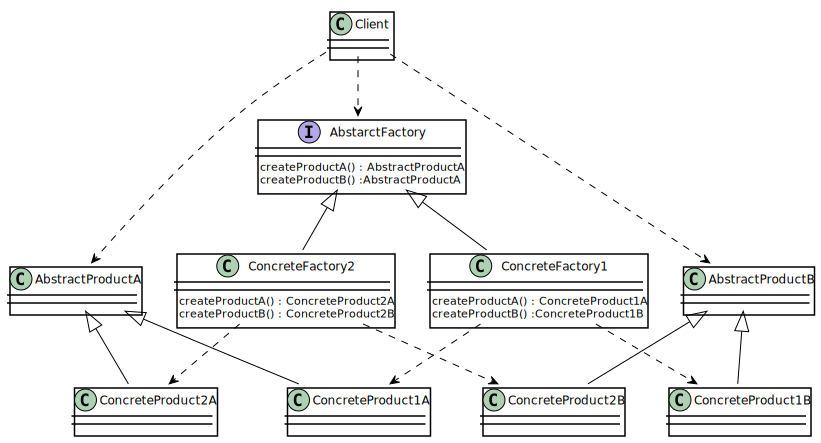
\includegraphics[width=\textwidth]{../out/diagrams/factory/flex}
\end{FIGURE}

\textbf{Участники:}
\begin{itemize}
	\item \emph{AbstractFactory} - интерфейс предоставляющий действия для других фабрик
	\item \emph{СoncreteFactory} - классы (ConcreteFactory1,ConcreteFactory2) выполняющий создание продуктов А1 и B1
	\item \emph{AbstractProduct} - абстрактный объект (AbstractProductA,AbstractProductB) реализующий объект
	\item \emph{ConcreteProduct} - классы (ConcreteProduct1A,ConcreteProduct1B,ConcreteProduct2A,ConcreteProduct2B)  реализующие классы объекты
	\item \emph{Client} - класс пользующийся интерфейсами,которые объявлены в AbstractFactory и AbstractProduct
\end{itemize}


\section{Способ применения}
Данный паттерн применим для систем сборки проектов под разные платформы, также его можно использовать для подключений к базе данных.
\chapter{Одиночка}
Одиночка — это порождающий паттерн проектирования.
\section{Назначение}
Гарантирует, что у класса есть только один экземпляр, и предоставляет к нему глобальную точку доступа.
\section{Структура}

\begin{FIGURE}[h]{Структура паттерна абстрактная фабрика\label{fig:example-figure}}
	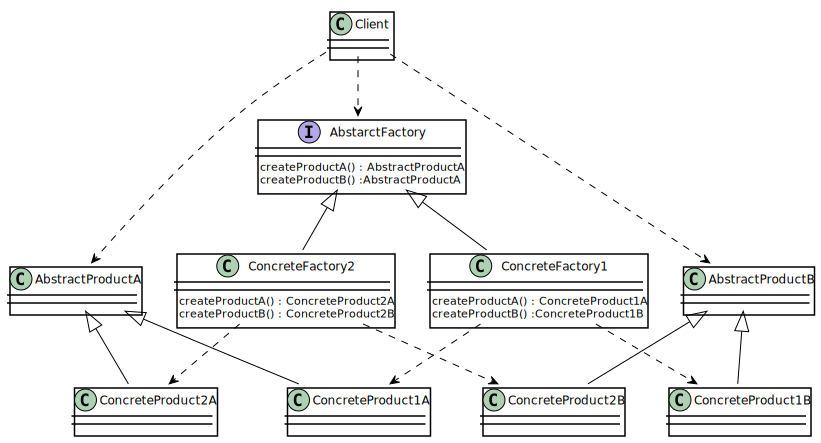
\includegraphics[width=\textwidth]{../out/diagrams/factory/flex}
\end{FIGURE}

\section{Способ применения}
Данный паттерн применим когда в приложении есть глобальное состояние и данное состояние находится в одинственном экземпляре
\chapter{Реализация паттернов}

\section{Диаграмма классов}
\begin{FIGURE}[h]{Диаграмма классов \label{fig:example-figure}}
	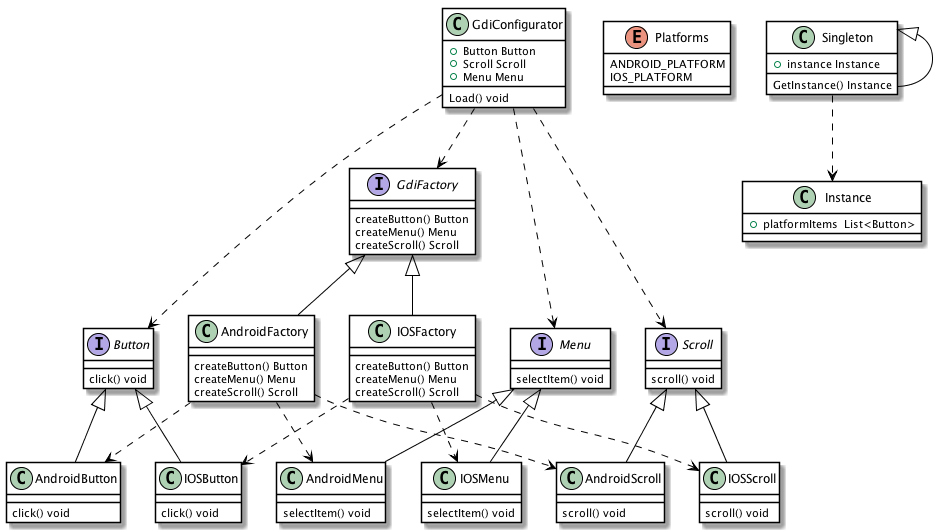
\includegraphics[width=\textwidth]{../out/diagrams/factory-go/factory-go}
\end{FIGURE}

\textbf{Участники:}
\begin{itemize}
	\item \emph{GdiConfigurator} - класс имеющий в себе продукты фабрики и использующий по назначению
	\item \emph{GdiFactory} - интерфейс определяющий стандартизированное поведение для фабрик
	\item \emph{IOSFactory} - конкретная фабрика для создания объектов  (IOSButton,IOSScroll,IOSMenu)
	\item \emph{AndroidFactory} - конкретная фабрика для создания объектов  (AndroidButton,AndroidScroll,AndroidMenu) 
	\item \emph{Scroll,Menu,Button} - интерфейсы определяющие стандартизированное  поведение объектов 
\end{itemize}


\section{Диаграмма последовательности }

\begin{FIGURE}[h]{Диаграмма последовательности\label{fig:example-figure}}
	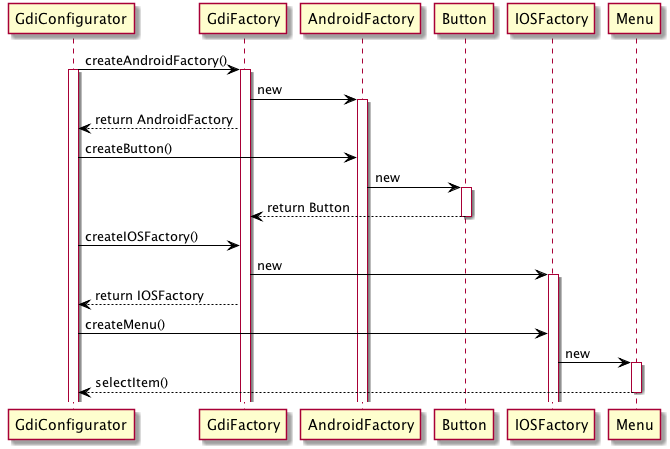
\includegraphics[width=\textwidth]{../out/diagrams/seq-go/seq-go}
\end{FIGURE}



\section{Код программы }

Ссылка на github \url{https://github.com/vinogradnick/Pattern_AB_Factory_Singleton}

\lstset{extendedchars=\true}

\begin{lstlisting}[language=Go]
package main

import (
"container/list"
"fmt"
)

const (
ANDROID_PLATFORM = 1
IOS_PLATFORM     = 2
)

type (
Button interface {
click()
}
Scroll interface {
scroll()
}
Menu interface {
selectItem()
}
GdiFactory interface {
createButton() *Button
createMenu() *Menu
createScroll() *Scroll
}
)

/*
---------------------------------------------------------------
IOS IMP
*/
type IOSFactory struct {
}

func NewIOSFactory() GdiFactory {
var g GdiFactory
g = IOSFactory{}
return g
}

func (I IOSFactory) createButton() *Button {
var b Button = IOSButton{}
return &b
}

func (I IOSFactory) createMenu() *Menu {
var m Menu = IOSMenu{}
return &m
}

func (I IOSFactory) createScroll() *Scroll {
var s Scroll = IOSScroll{}
return &s
}

type (
IOSButton struct {
}
IOSMenu struct {
}
IOSScroll struct {
}
)

func (I IOSButton) click() {
fmt.Println("click from ios button")
}
func (I IOSScroll) scroll() {
fmt.Println("scroll from ios scroll")
}
func (I IOSMenu) selectItem() {
fmt.Println("selectItem from ios menu")
}

/*
---------------------------------------------------------------
Android IMP
*/
type AndroidFactory struct {
}

func (I AndroidFactory) CreateButton() *Button {
panic("implement me")
}

func NewAndroidFactory() GdiFactory {
var g GdiFactory
g = AndroidFactory{}
return g
}
func (I AndroidFactory) createButton() *Button {
var b Button = AndroidButton{}
return &b
}

func (I AndroidFactory) createMenu() *Menu {
var m Menu = AndroidMenu{}
return &m
}

func (I AndroidFactory) createScroll() *Scroll {
var s Scroll = AndroidScroll{}
return &s
}

type (
AndroidButton struct {
}
AndroidMenu struct {
}
AndroidScroll struct {
}
)

func (I AndroidButton) click() {
fmt.Println("click from android button")
}
func (I AndroidScroll) scroll() {
fmt.Println("scroll from android scroll")
}
func (I AndroidMenu) selectItem() {
fmt.Println("selectItem from android menu")
}

/*
------------------------------------------------------
GDI Configurator
*/
type GdiConfigurator struct {
Button Button
Menu   Menu
Scroll Scroll
}

func NewGdiConfigurator(platform int) *GdiConfigurator {
var f GdiFactory
switch platform {
case ANDROID_PLATFORM:
f = NewAndroidFactory()
case IOS_PLATFORM:
f = NewIOSFactory()
}
return &GdiConfigurator{
Button: *f.createButton(),
Menu:   *f.createMenu(),
Scroll: *f.createScroll(),
}

}
func Load(conf *GdiConfigurator) {
conf.Scroll.scroll()
conf.Button.click()
conf.Menu.selectItem()
}

/*
Signleton
*/
type singleton struct {
platformItems list.List
}

var instance *singleton

func GetInstance() *singleton {
if instance == nil {
instance = &singleton{} // Это НЕ потоко-безопасно
instance.platformItems.Init()
}
return instance
}
func printList(items list.List) {
for e := items.Front(); e != nil; e = e.Next() {
fmt.Println("%#v", e.Value)
}
}
func main() {
c := NewGdiConfigurator(IOS_PLATFORM)
Load(c)
GetInstance().platformItems.PushBack(c.Menu)
printList(GetInstance().platformItems)
}


\end{lstlisting}

\end{document}
